%&pdflatex
\documentclass{article}

\usepackage{color}
\usepackage{subcaption}
\usepackage{graphicx}
\usepackage{multicol}
\usepackage{geometry}
 \geometry{
 a4paper,
 total={170mm,257mm},
 left=20mm,
 top=20mm,
 }

 \newenvironment{Figure}
  {\par\medskip\noindent\minipage{\linewidth}}
  {\endminipage\par\medskip}

\newcommand{\toolname}{{\color{blue}TOOL\_NAME }}


%Titles:
%\title{The Evolution of National AS Chokepoints and Their Connection to
%Internet Freedom}
\title{Borders and Gateways: Measuring and Analyzing National AS Chokepoints}


\graphicspath{{./images/}}
\setlength{\parskip}{0pt}

\begin{document}
\maketitle
\begin{multicols}{2}

  \section{Abstract}

  Internet topology has been measured and modeled for many years, but few studies  quantify how the topology changes over time.  Over the past decade, governments around the world have recognized that the Internet is a powerful tool for controlling and surveilling their citizens, and they have begun enacting common policies for ASes operating within their borders.

  In this paper, we ask how AS topology has changed over time with respect to national boundaries.  We introduce a new measure, \emph{chokepoint potential}, to characterize how a country's AS topology is organized in terms of paths that can carry traffic across international borders.  To study country-level chokepoints, we developed \toolname, a suite of open source, cross platform, and efficient tools for monitoring national chokepoints on the AS graph.  To illustrate these ideas and tools, we studied how chokepoint potential correlates with two independent measures of civilian liberty, finding [NEED A RESULT HERE].  [NEED A RESULT FOR WHAT WE FOUND FOR EVOLUTION OVER TIME].

This paper extends earlier research on AS topology and BGP simulation to study chokepoints across the Internet over multiple years, using our
path simulation and routing tree datasets to view snapshots of the Internet
over multiple years. We provide comprehensive and accessible tools for studying
the complex and dynamic AS level Internet topology. Through this approach we
can more carefully evaluate the state of the Internet than was previously possible. 

%% Paths on the Autonomous Systems (AS) graph of the Internet
%% derived from the Border Gateway Protocol (BGP) can be used by researchers to
%% understand the dynamics of Internet topology and to interpret how that
%% topology may enable nations to enact censorship, surveillance, or other
%% Internet control measures. Unfortunately datasets of these paths are not
%% generally made publicly available, and paths collected from measurements such as
%% traceroute or BGP probes tend to be incomplete. Simulation
%% frameworks have been used to generate AS paths based on inferred AS relationships.
%% We introduce \toolname, a suite of open source, cross platform, and efficient
%% tools for monitoring national chokepoints on the AS graph. We introduce chokepoint potential as an important measure of a nation's ability to 
%% control Internet traffic, either through censorship or surveillance.
%% Previous research endeavors in this
%% direction have only identified chokepoints in single snapshots. We apply our
%% path simulation and routing tree datasets to view snapshots of the Internet
%% over multiple years in order to introduce a new technique to investigate the
%% evolution of the complex and dynamic AS level Internet topology. Through this approach we
%% can more carefully evaluate the state of the Internet than was previously possible. As an
%% application of \toolname we compare Freedom House's Freedom On The Net (FOTN) score for
%% Internet freedom and with our chokepoint potential measure in order to interpret
%% the relationship between AS-level topology and actual censorship activity, providing an
%% illustration of new ways to monitor which governments can easily control the flow of 
%% information in their nations and whether they are acting on that potential.

\section{Introduction}

\par Widespread Internet censorship and surveillance pose a
significant threat to individuals throughout the world. As routine
tasks, communications, entertainment, and information move on-line and
are mediated by the Internet, most of us have little choice about
whether or not to rely on the Internet.  According to the
International Telecommunication Union (ITU), the number of individual
Internet users increased from 1.024 million in 2005 to 3.578 million
in 2017 \cite{itu}. The majority of these users operate in an
environment that restricts Internet freedom in some way. For example,
the 2017 Freedom on the Net report from Freedom House reports that
64\% of Internet users belong to a nation with Internet that is not
free or partly free \cite{FOTN}.  Beyond censorship and surveillance,
the EU is considering content rules surrounding copyright, net
neutrality rules in the U.S. were recently overturned, and large
content delivery networks are under enormous pressure to 'do
something' about fake news and bad actors. Taken together, these
trends will likely restructure the Internet in unforeseen ways,
as organizations respond to new challenges and realities.

Today, most such control is exercised at the country level,
as governments have recognized both the threat and the opportunity
that is posed by ubiquitous on-line communication. For example, much
of the organization, revolutionary momentum, and broadcasting of
events during the Arab Spring have been attributed to social media
communications through the Internet \cite{arabspring}, and similarly several countries
sought to control these movements by disconnecting in-country networks from the rest of the world (FIXME: need references here).

These two factors, increasing levels of content monitoring and
Internet dependence, point to the need for improved tools and methods
for studying worldwide Internet censorship and surveillance over time.
[A SENTENC OR TWO HERE SUMMARIZING THE STATE OF THE FIELD AND WHAT'S
  MISSING.]  In this paper, we focus on AS-level topology and on
censorship, asking how AS topology has changed over time with respect
to national boundaries.  We define \emph{chokepoint potential} to
quantify how a country’s AS topology is organized in terms of paths
that can carry traffic across international borders.  We developed a
suite of tools, called \toolname, for studying national chokepoints on
the AS graph efficiently. To illustrate these ideas and tools, we
study how chokepoint potential correlates with two independent
measures of civilian liberty, finding [NEED A RESULT HERE]. [NEED A
  RESULT FOR WHAT WE FOUND FOR EVOLU- TION OVER TIME].

The paper extends earlier research on AS topology, first by introducing the chokepoint potential measure, then by presenting open-source cross-platform tools for simulating
and Border Gateway Protocol (BGP) networks, determining chokepoint potential at the country level, and analyzing how this measure has changed over time for certain countries of interest.


%Whether or not AS-level topology supports
%these efforts is a research question pivotal to an understanding of
%the dynamics of Internet censorship and surveillance.

%% \par
%% The Internet has been used as a tool for the citizens of authoritarian nations to voice opinions,
%% organize revolutionary movements, and connect with other nations' governments and citizens
%% to seek aid. Much of the organization, revolutionary momentum, and broadcasting
%% of happenings during the Arab Spring can be attributed to social media communications
%% through the Internet \cite{arabspring}. Because of this potential, national governments may
%% take interest in maximizing their ability to control the flow of information on the Internet.
%Censorship and Surveillance are growing phenomena

%The Internet is Dynamic and growing

We are interested in how AS topologies have changed as the total size of the graph has grown from about 10,000 nodes in the early 2000s to over 60,000 today.
The structural
properties of national AS graphs have evolved differently
from nation to nation whether from economic decision making, infrastructural necessities, or
efforts to build a powerful censorship and surveillance
network.
%The Autonomous Systems (AS) layer of the Internet has grown and changed dramatically over its history.
%The locations and relationships of these ASes determine how many chokepoints
%of AS-level routing exist and what strength these chokepoints have in regards to paths intercepted.
This rapid expansion, together with the changing role of national
governments, points to the importance of understanding properties like
path robustness, AS hierarchies, and the potential for organizations to
control information as it flows in and out of their networks.

%Current Events

%Diverse Censorship Architecture
\par Every nation has a different layout and count of ASes. The
censorship and surveillance strategies of nations also differ. For
instance, China both conducts keyword filtering in border ASes and in
internal provincial nodes \cite{chinafiltering}, while Iran routes its
Internet traffic through a centralized facility \cite{irancensor}.
Having views into the AS topology of a nation, then, will both help
researchers identify nations that could easily conduct censorship and
also provide possible insight into what kind of censorship is likely
being conducted. The measure of chokepoint potential, defined later in
this paper, is a succint way to estimate the important properties of
border ASes related to these capabilities.

% Major Contributions
\par
The primary contributions of our work are as follows: \textbf{1.} We introduce the measure of chokepoint potential and 
motivate its value as way to interpret the capability for a nation to enact censorship of its Internet traffic. \textbf{2.} We
provide an overview of the evolution of national AS-level chokepoints over time, showing the evolution of the Internet
allowing for a comparision between nations. \textbf{3.} We develop a new tool, \toolname, that provides the capability for
efficiently evaluating chokepoints for a given state of the Internet. Finally, \textbf{4.}, we show that our chokepoint measure
has a significant relationship to Internet freedom as measured by a qualitative source.


% Rest of Paper Layout
\par
The layout of the rest of this paper is as follows: Section 3 provides relavent background information
to the problems we are investigating; Section 4 introduces and defines the measure of chokepoint
potential; Section 5 details our tool for simulating and evaluating AS topologies \toolname; Section 6
explains our experimental setups; Sections 7, 8, and 9 provide results, discussion, and related work
respectively.

\section{Background}

The AS-layer of the Internet is the highest level of organization of the Internet. ASes generally represent ISP networks,
large university networks, or government entities. Interdomain routing between these ASes is governed by BGP, and
individual ASes may have local preferences for how they wish to send packets along, but they cannot govern the paths
selected by other ASes. AS topology researchers often use measurement tools to create a picture of the global Internet.
These measurement tools, for instance BGP Updates from BGPStream \cite{BGPStream} or empirical paths from traceroute, suffer from
incompleteness and innacuracies \cite{tracerouteProblems}.
\par
AS-level studies are further complicated by the lack of ground truth data for AS relationships and BGP paths. For AS relationships,
inference is often used based on economic considerations to classify the relationships of ASes. This was first done by Gao \cite{gao} by
maximizing the occurances of certain economic rules on the AS graph by choosing a particular set or relationships. This technique was only
evaluated against a single ISPs set of true relationships, however. As part of the CAIDA project, this inference technique was extended, leading
to the CAIDA AS-relationship dataset \cite{CAIDApaper}, \cite{CAIDA}. We choose these relationships for our purposes, and they are the current
research standard.
\par
Finding BGP paths is more of a challenge. Packet based simulations, wherein BGP is simulated directly, are computationally infeasible for the
scales relevant to a global study. An accurate, but realistic, simulation technique must be chosen to provide useful research potential in this regard.
The BGPSim algorithm \cite{quicksand} is one such simulation technique that is suitable for this study's purposes. BGPSim takes a set of AS relationships
as input, such as those provided by the CAIDA dataset \cite{CAIDA}, and returns routing trees based off of these relationships. These paths are found via
a modified breadth-first seach (BFS) algorithm. The BFS adds edges to routing trees first according to local preference (LP), then shortest path (SP), and finally tiebreak (TB).
A resulting routing tree contains all the equally reasonable paths (according to economic concerns) that exist between source ASes (within the routing tree) to 
destination ASes (the root of the routing tree). We find this technique suitable for our purposes, so we extend BGPSim 
(in ways explained further in this paper) as part of \toolname.

\section{Chokepoint Potential}

\begin{Figure}
	\centering
	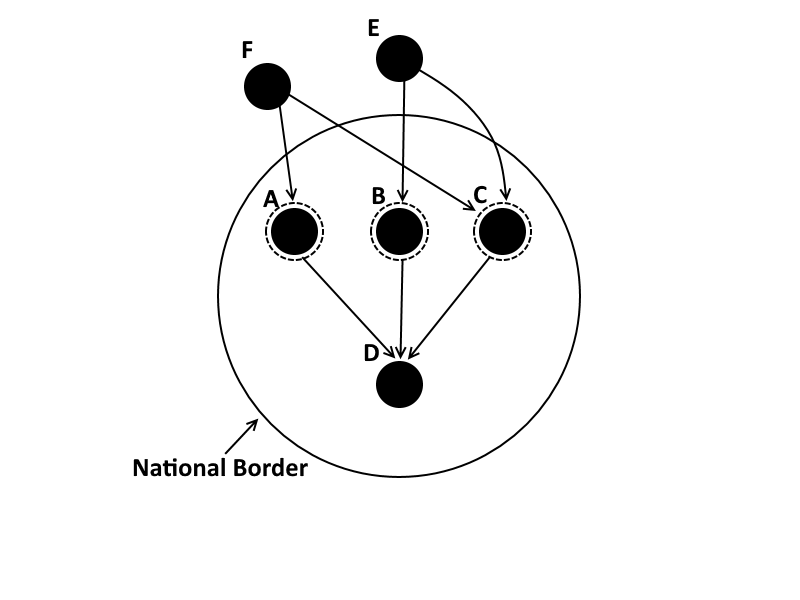
\includegraphics[width=\linewidth]{chokepoint}
	\captionof{figure}{Chokepoint potential example. ASes A,B, and C are all border nodes. 
						AS D is an internal node. ASes E and F are both external nodes.
						The out-to-in chokepoint potentials of A,B, and C are 0.25, 0.25, and 0.5 respectively.}\label{fig:chokepoint}
\end{Figure}

% Why Border ASes?
In order to identify AS chokepoints and compare nations, we need a measure that can be calculated from the many paths between
ASes. First, we decided to use a measure that is evaluated only on border ASes, or ASes that lie one hop from an AS belonging to another nation. 
We argue that this is intuitive because border
ASes are the first opportunity for nations to censor incoming traffic and the last opportunity for nations to block access to
foreign websites from within their borders. Additionally, while internal chokepoints may intercept many paths, those paths are required
to have entered through a border AS (in the case of out-to-in paths) or exit through a border AS (for in-to-out paths). This simplification has
the added benefit of making calculations more efficient.

% What is our measure, why does it make sense?
\par
We define the chokepoint potential of a border node to be the ratio of paths intercepted by that border node
to the number of paths intercepted by all other border nodes. Consider a border node $b$, belonging to country $c$.
If $P_c$ is the set of paths in to or out of country $c$ and $B_p$ is the set of border nodes within path $p$, then the
chokepoint potential of $b$, $CP_b$ is defined formally in equation \ref{eqn:chokePointPotential}. This measure captures
the relative strength exhibited by a border nodes in regards to what portion of paths it intercepts. This is calculated
seperately for in-to-out paths (those starting from a source in the country in question) and out-to-in paths.

% Formal Definition
\begin{equation}\label{eqn:chokePointPotential}
CP_b = \frac{|\{p \in P_c \textrm{ s.t. } \{b\} \subseteq B_p\}|}{\sum_{p \in P_c}|B_p|}
\end{equation}

\par
Given a set of BGP paths, this measure is an intuitive way to compare individual ASes and different nations. With this measure,
the chokepoint potential sum over all border nodes for a country is 1.0, as in, all of the border nodes collectively control the
flow of information over the nation's border. To compare one nation to another, we can inspect how many border nodes minimum are required
to obtain a certain chokepoint potential. The more border nodes required, the more difficult it would be for that nation to perform
censorship or surveillance. This is a clear way to differentiate nations based on the topology of their ASes.

\section{\toolname}

% Preprocessing and Data pipeline
\toolname is a new tool that calculates the chokepoint potential for every border AS given a set of AS relationships.
\toolname first takes the entire AS graph, as in from the CAIDA dataset \cite{CAIDA}, and uses the principles of BGPSim \cite{quicksand}
to generate a set of routing trees. These routing trees, as well as a set of AS country codes (for identifying which nation an AS belongs to)
are used to determine the chokepoint potentials for every border node. In our experiments, we used the country codes returned from Team Cymru's
IP to ASN whois service \cite{cymru}.

% Routing Tree Algorithm
\par
In order to calculate the routing trees, we use an extended version of the BGPSim algorithm developed by Gil et. al in \cite{quicksand}. In
our work we addressed the following limitations of BGPSim: (1) BGPSim returns a set of ASes for each path it considers but not the order in which
they are visited; (2) Once routing trees are determined, they cannot be accessed later without recalculation; (3) BGPSim relies on the outdated parallelization
framework DryadLinq for C\#. To address these issues, we use a Python implementation we dub BGPSimPy. BGPSimPy returns ordered paths from its routing trees,
saves routing trees to disk after calculation, and is parallelized with MPI via the mpi4py library. These improvements have the added benefit of yielding a cross platform
routing tree algorithm that is ready to work on most hardware.

% Chokepoint calculation
\par
Once BGPSimPy generates the routing trees, they can be processed to determine chokepoint potentials. This is done by iterating over every path between each AS-pair. Because
we use the same random tie-break as BGPSim, there is only 1 path between each AS-pair considered, even if multiple exist in the routing tree. Once a path is determined, it is
traversed. For each node visited, the number of paths intercepted by that node is incremented. This is done for both in-to-out paths and out-to-in paths, so only one traversal is
necessary per path. Additionally, the number of paths of each type that belong to each nation is tallied, as this makes up the denominator in equation \ref{eqn:chokePointPotential}.

\section{Experimental Setup}

% Chokepoint Evolution
There is ongoing research interest into ASes that intercept large portions of Internet paths \cite{throats}, \cite{decoy}. Some questions remain unanswered however. For instance, to what
extent does the current state of the Internet support national governments' attempts to censor Internet traffic? How does this vary from nation to nation? Is the Internet developing more
powerful chokepoints, or becoming more evenly accessible?
\par
To probe these questions we first used our chokepoint evaluation technique to investigate the chokepoint potential of all nations for the current Internet as well as the
change in chokepoint potentials over time. We looked at multiple snapshots of AS relationships from the CAIDA dataset (2012-2018).
For each timestamp, we generated routing trees based on these relationships. Then we calculated the chokepoint potential for every border node per snapshot. As a result we can investigate
how countries have changed overtime in their capability to enact censorship and surveillance. This is an attempt to understand what topological trends have developed historically.
With this test we can compare nations, and see which ones have overtime increased their capability to control the flow of information across their borders.

% Chokepoints and Internet Freedom
If chokepoint potential can be leveraged to determine if a nation can easily implement censorship, it stands to reason that their might already be a negative relationship between
the chokepoint potential of a nation and its Internet freedom. If a significant relationship were to be found it would strengthen chokepoint potential as a measure of a nation's censorship capability
and it would increase the value in monitoring chokepoint potentials across the globe.
\par
We tested whether a significant relationship exists between our measure of national chokepoints and a qualitative evaluation of Internet Freedom. For Internet Freedom we used
the Freedom House's Freedom On The Net report \cite{FOTN}. FOTN scores quantify the level of Internet freedom in countries. Each country receives a numerical score from 0 (the most free)
to 100 (the least free).
 To evaluate our measure, we first must define a way to rank each nation in regards to our chokepoint potential measure.
Acharya et al. \cite{throats} chose to determine how many ASes were needed (globally) to intercept 90\% of paths as a measure of the AS hierarchy. We choose a similar measure. Because we are
looking at national comparisons, however, we record how many border ASes are required to incercept 90\% of in-to-out or out-to-in paths for each nation. We compared this number
with each nation's (of those recorded by Freedom House) freedom on the net score.

\section{Results}
\subsection{Nations Over Time}

\begin{Figure}
	\centering
	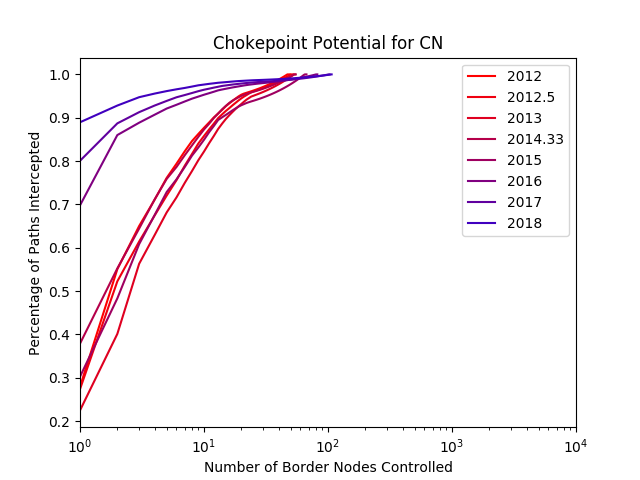
\includegraphics[width=\linewidth]{single_CN}
	\captionof{figure}{The evolution of China's in-to-out Chokepoint Potential}\label{fig:ChinaChokePoint}
\end{Figure}

\begin{Figure}
	\centering
	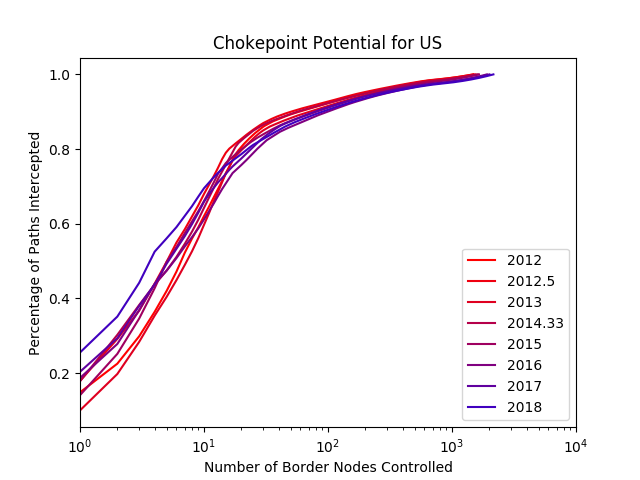
\includegraphics[width=\linewidth]{single_US}
	\captionof{figure}{The evolution of the US's Chokepoint Potential}\label{fig:USChokePoint}
\end{Figure}

To inspect the changes over time for each nation we arrange all the border nodes belonging to a nation into a list. The list of border ASes is reverse sorted
so that the first AS has the highest chokepoint potential. The sum of all these nodes' chokepoint potential is 1.0. Then we step through the list, and record
the cumulative chokepoint potential of all the ASes seen so far. If we plot the number of ASes controled vs the cumulative chokepoint potential for that number
of ASes, we can see how many ASes are required for a certain nation to control different percentages of paths. We repeat this process for each snapshot to highlight
changes over time.

\par
For instance, consider figures \ref{fig:ChinaChokePoint} and \ref{fig:USChokePoint}. 
The x-axis (log-scale, so that countries with large differences in AS counts can be compared more easily)
is the number of border nodes controlled, and the y-axis is the ratio of in-to-out paths intercepted. Each line represents a different snapshot, with the more red lines being
farther in the past and more blue lines being more recent.

\par
The United States and China are shown here to exhibit their dramatic differences. First, it is worth pointing out that the United States has many more ASes than China, hence
it's line extends further to the right in these plots. We also see that China, in all cases, can control a much larger portion of its paths with much fewer ASes than the
United States. This result is entirely expected. Of more interest is the trends that can be seen over time. China clearly has developed an AS topology such that very few
ASes can intercept nearly all BGP paths. The US has evolved in a different way. While it has become somewhat easier for the US to intercept most of its paths, it has become
more difficult to intercept around 70\% of its paths and higher. This suggest an expansion of ASes on the interior and more connections, as well as a strengthening of
the very top ASes.

\begin{Figure}
	\centering
	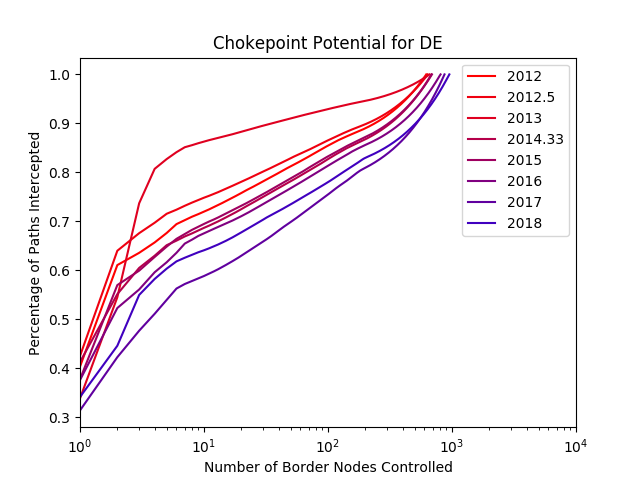
\includegraphics[width=\linewidth]{single_DE}
	\captionof{figure}{The evolution of Germany's in-to-out Chokepoint Potential}\label{fig:GermChokePoint}
\end{Figure}

\par
Not all nations have evolved to a state where it easier to control paths. One example is Germany, as shown in figure \ref{fig:GermChokePoint}. For Germany, a fairly constant
trend shows that it has become more difficult to intercept BGP paths. Unlike the other examples, any amount of German border ASes intercept less paths in more recent tests.

\begin{Figure}
	\centering
	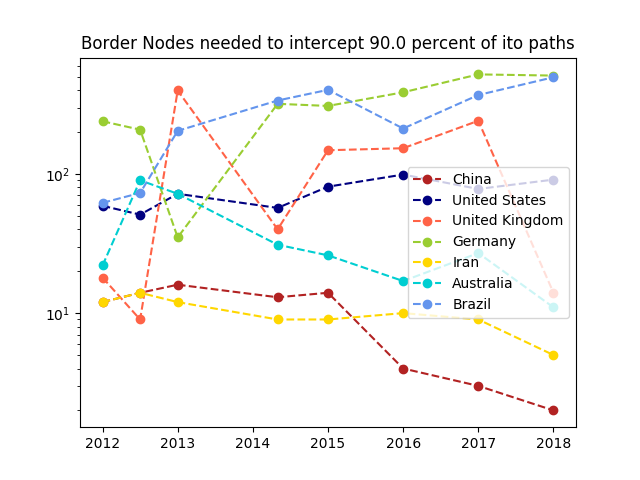
\includegraphics[width=\linewidth]{NodesNeeded}
	\captionof{figure}{Number of ASes to intercept 90\% of ito paths for multiple nations over time}\label{fig:nodes}
\end{Figure}


\par
In order to compare multiple nations, we have plotted the number of ASes needed to intercept 90\% of in-to-out paths
for each timestamp recorded. These results are detailed in figure \ref{fig:nodes}.
The distinct behaviors of each nation are rather striking. We can see a steep decline for some
nations known to limit Internet freedom (China and Iran) as well as the increase for other nations
(Germany and Brazil). Other nations have stayed more stable. It is worth pointing out that if a nation
has required the same number of border ASes to control many paths over several years, this suggests
that the chokepoints have grown to intercept more paths. The reason for this is that the number of ASes,
and thus the number of paths, has increased globally over time. This fact makes the decline in ASes
needed for some nations even more glaring.


\subsection{Internet Freedom}

In our test of the relationship between Internet Freedom and chokepoint potential, we plotted the Freedom on the Net score
of each nation vs the number of border ASes that that nation needed to in order to intercept 90\% of in-to-out paths. Additionally,
we evaluated the relationship with an Ordinarly Least Squares (OLS) fit, and found that the relationship was statistically significant,
with a p-value $\leq$ 0.002 for 2017. The relationship held for other timestamps as well. The results for 2017 are shown in figure \ref{fig:fotn2017}

\begin{Figure}
	\centering
	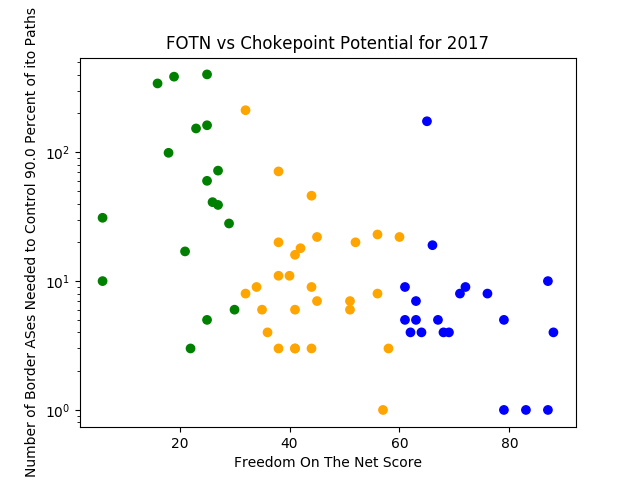
\includegraphics[width=\linewidth]{fotn2017}
	\captionof{figure}{Number of ASes to intercept 90\% of ito paths vs Freedom On The Net Score (2017)}\label{fig:fotn2017}
\end{Figure}

\par
For each timestamp we see what appears to be two general modes of behavior. Nations that are not free or partly free tend to requrie few ASes
to intercept 90\% of their paths. Free nations on the otherhand require varying degrees of large numbers of ASes to control the same portion
of their paths. There are interesting outliers for both situations, however. Countries like Estonia (EE) or Iceland (IS) are very free but require
few nodes to control most of their paths. The reason for these outliers is likely that their overall AS counts are very low. On the other hand, Russia (RU)
is a very interesting outlier in that it is found to be not free by FOTN, but requires a large number of ASes to control most of its paths. This suggests
that the censorship efforts in Russia might be of types that do not require AS level chokepoints.

\section{Related Work}   
\par
Previous studies have used BGP path models to find ASes that
intercept a high fraction of paths. One such project in \cite{throats}
identified that 90\% of paths on the Internet could be intercepted with only 30
or so ASes. The researchers in \cite{throats} generated paths by first using
only paths to top websites as defined by the Alexa top websites project,
and then appending additional edges to those paths from the full
AS graph according to the principles defined by Gao \cite{gao}. Many of the
ASes that were found to intercept a large number of paths were found to be
within nations that conduct censorship. As an extension of these results,
another paper \cite{decoy} revealed that ASes that intercept many paths could
be utilized for decoy routing. This approach for identifying AS level
chokepoints has several potential pitfalls that are remedied by the approach
taken in this paper. First, the authors in \cite{throats} didn't consider that
many of the paths found from the Alexa top websites would have destinations in
nations that censor Internet traffic, particularly China due to its large
Internet population. This artificially inflates the chokepoint nature of
Chinese ASes. As an alternative, in this paper we consider paths from every
source-destination AS pair, and we make a distinction between in-to-out paths
and out-to-in paths. Secondly, chokepoints have previously only been
identified at a single snapshot of the Internet. This makes it difficult to
discuss the evolution of Internet topology, and whether or not chokepoints are
anomalous or common. Finally, the aforementioned approach for identifying
chokepoints does not allow a clear comparison between different nations. It
can be said that one nation controls a large portion of Internet paths, but
not how easily traffic directed through that country could be intercepted on a
national level. For this, some aggregate measure across all of the border ASes
within a country must be considered, as it is in this paper.     
\par
In \cite{chinafiltering}, Xu et al. investigated the AS level topology of China
to identify where keyword filtering occurred. They found that the most
effective ASes with which to deploy keyword filtering devices are those in the
backbone of the Chinese AS topology. A relevant contribution of
\cite{chinafiltering} is that, while most filtering occurs in border ASes,
some filtering is controlled by non-central provincial ASes. China has a
diverse strategy for Internet censorship, both targeting chokepoints and the
Chinese provincial network. The potential for various forms of censorship in
regards to various AS level topologies motivates the question: Is centralized
censorship or decentralized censorship more common? Instead of directly
identifying censorship devices on the AS graph, we instead quantify the
chokepoint potential of ASes on the national level, and then compare that with
qualitative Internet freedom measures and empirical censorship events.
\par
We are not the first to investigate the relationship between Internet freedom and
AS-level topology. Similar techniques have been used to classify nations according
to the connectivity of their ASes \cite{politicsrouting}. This has only been done for a
single moment in time, however, making the results limited in terms of stability and predictability.
Additionaly, previous work has not used country level chokepoints as the link between Internet topology
and censorship or surveillance practices. The work in \cite{politicsrouting} chose to relate Internet topology
to the Freedom of the Press measure from freedom house instead of the Freedom On The Net score. They chose to do this
to include more nations. Additionally, this study didn't include the United States and Russia in their experiments because they were
outliers in regards to their topologies. Through our approach we hope to extend this previous work by finding an interesting measure for
understanding the dynamics of all nations, as well as targeting our results more specifically to Internet freedom by using the Freedom On
The Net score as our measure for Internet freedom. Through our techniques, we provide a simple measure that not only 
sheds light on the relationship between topology and Internet freedom, but reveals currently free
nations that could easily implement censorship if their governments decided to.


\section{Discussion}

% Chokepoint Potential
In this paper we have introduced a novel measure, chokepoint potential, that allows us to
evaluate the level of difficulty that a government faces when trying to censor the Internet
based entirely on AS-level topology. Our technique for evaluating chokepoint potential using
\toolname provides a monitoring capability of BGP dynamics that was previously not possible.
We have taken advantage of efficient simulation, standard AS relationship datasets, and cross-platform
design principles so that this tool is readily deployable for future research.
% Ecolution over time
\par
Our application of \toolname to investigate evolutions in the global AS graph over time shows us
interesting trends in AS topologies.
% Internet Freedom
\par
We have validated chokepoint potential as having a relationship to actual censorship by showing
the significance of the relationship between the chokepoint potential of nations and their FOTN
score from freedom house.

\subsection{Routing Trees Dataset}
In the hope to further AS topology research, we have open sourced the routing tree datasets generated in this study. While we generated routing trees
with an efficient algorithm, it still requires considerable time to calculate them, particulary for multiple timestamps. Additionally, each set of routing trees
takes up on the order of 50GB of disk space. By releasing these datasets we hope that researchers looking for a particular set of routing trees will find
working with these simpler than recalculating them. This also provides an alternative to research projects that might otherwise use measurement tools to estimate
BGP paths.

% Points of Presence


\subsection{Future Work}
% OONI data
While linking chokepoint potential to FOTN scores is a substantial contribution, it still stands that FOTN can serve only as a proxy for censorship.
This is useful for large trends and general understanding, but a more fine-grained approach could be used to interpret the direct connection between
actual censorship events and the shifts in the AS graph. The Open Observatory of Network Interference, or OONI, \cite{OONI} provides Internet users around
the world with a tool called the ooniprobe. The ooniprobe lets users run a suite of tests to identify censorship anamolies of various types, and the results are
recorded in the large OONI database. Matching up changes in OONI measurements, such as increased censorship campaigning in an authoritarian nation, with shifts
in chokepoint potential would be a major step in understanding the interplay of censorship and AS-level chokepoints. This process involves designing a way to classify
censorship events and chokepoint potential changes, and as such lies beyond the scope of this study.

\bibliographystyle{plain}
\bibliography{paper}

\end{multicols}

\end{document}
